\documentclass[11pt,a4paper]{article}

\usepackage[T1]{fontenc}
\usepackage[utf8]{inputenc}
\usepackage{lmodern}
\usepackage[english]{babel}
\usepackage{microtype}

\usepackage[a4paper,margin=2.7cm]{geometry}
\usepackage{graphicx}
\usepackage{booktabs}
\usepackage{tabularx}
\usepackage{enumitem}
\usepackage{listings}
\usepackage{xcolor}
\usepackage{caption}
\usepackage[hidelinks]{hyperref}
\usepackage{cleveref}

\setlist{itemsep=2pt, parsep=0pt, topsep=4pt}

\definecolor{codebg}{gray}{0.96}
\definecolor{codekw}{RGB}{0,80,140}
\definecolor{codecm}{RGB}{100,110,100}
\definecolor{stubgray}{gray}{0.45}

\lstset{
  basicstyle=\ttfamily\footnotesize,
  keywordstyle=\color{codekw}\bfseries,
  commentstyle=\color{codecm}\itshape,
  stringstyle=\color{black!70},
  backgroundcolor=\color{codebg},
  breaklines=true,
  breakatwhitespace=true,
  showstringspaces=false,
  frame=single,
  framerule=0pt,
  xleftmargin=8pt,
  aboveskip=8pt, belowskip=8pt,
  captionpos=b,
}

\lstdefinelanguage{json}{
  morestring=[b]",
  morecomment=[l]{//},
  literate=
    *{:}{{{\color{codekw}:}}}{1}
     {,}{{{\color{codekw},}}}{1}
     {\{}{{{\color{codekw}\{}}}{1}
     {\}}{{{\color{codekw}\}}}}{1}
     {[}{{{\color{codekw}[}}}{1}
     {]}{{{\color{codekw}]}}}{1},
}

% Marca una sezione non ancora scritta. Va tolto il comando, non solo le
% occorrenze, prima della consegna: se \stub non esiste piu', un residuo
% non compila invece di passare inosservato.
\newcommand{\stub}[1]{%
  \par\medskip\noindent{\color{stubgray}\itshape [to be written --- #1]}\par\medskip}

\title{VoltShare}
\author{}
\date{}

\begin{document}

\begin{titlepage}
\centering
{\large University of Pisa\par}
{\large Master's Degree in Artificial Intelligence and Data Engineering\par}
{\large Distributed Systems and Middleware Technologies\par}
\vspace{3.5cm}
{\Huge\bfseries VoltShare\par}
\vspace{0.6cm}
{\Large Project Documentation\par}
\vspace{0.4cm}
{\large A distributed coordination system for electric-vehicle charging stations\par}
\vfill
{\large Group members:\par}
\vspace{0.2cm}
{\large Andrea Innocenti \par Lorenzo Barci \par}
\vspace{1.2cm}
{\large Academic Year 2025/2026\par}
\end{titlepage}

\tableofcontents
\newpage

\section{Introduction}
\label{sec:introduction}

VoltShare coordinates a network of electric-vehicle charging stations. Drivers find a
station, reserve a connector, plug in and are billed; the operator sees the network from a
back office. Underneath, the system decides three things: which vehicle gets which connector,
how the limited electrical capacity of a site is shared among the cars charging at it, and
what happens to both when a node fails.

This domain represents a real contention scenario: different drivers could request the same connector at the same time. This problem cannot be resolved in an easy way by a central authority that assigns arbitrarly the driver
to a resource, because they have their own destination and can ignore any suggestion.
The system can only \emph{arbitrate the requests that drivers make}.


\subsection{The problems this project solves}

Four of them:

\begin{itemize}
  \item \textbf{Exclusive access to a physical resource.} Several drivers ask for the same
        connector at the same instant, and the outlet must end up promised to one of them.
  \item \textbf{One reservation per vehicle across the whole network.} This is the hard one.
        Two stations can each be locally correct and still break the guarantee together, so
        it needs an authority, which then needs replication, election and a quorum to
        survive its own failure.
  \item \textbf{Sharing a divisible resource.} Tipically, in a real word scenario, the total site capacity is lower than the sum of what its
        connectors are rated for, so the available power is apportioned among active
        sessions and renegotiated whenever a car arrives, leaves or fills up.
  \item \textbf{Failures that must not take resources with them.} Nodes crash and links
        break, and from the outside the two are indistinguishable. A reservation held by a
        node that has stopped answering must be released without waiting for it to return.

\end{itemize}

\Cref{sec:problems} states all seven problems precisely, \cref{sec:addressing} gives the
mechanism chosen for each, and \cref{sec:fault-tolerance} covers the failures.

The outlet, its contactor, its meter
and the car are an emulator speaking a reduced set of OCPP 1.6-J messages (see \cref{sec:api-ws-cp}), so the boundary
falls where a real interface already exists (\cref{sec:boundary}). Seven containers on one
host run everything else (\cref{sec:deployment}).

Measurements come from running deployments and where something was not measured, the text says so,
and the limits are declared in \cref{sec:no-tolerance}.

\section{Requirements Specification}
\label{sec:requirements}

Five parties take part, and the names in \cref{tab:actors} are used in this exact sense for
the rest of the document.

\begin{table}[h]
\centering\small
\renewcommand{\arraystretch}{1.15}
\caption{Actors. The charge point is a peer of the system; the browser is a client of it.}
\label{tab:actors}
\begin{tabularx}{\textwidth}{@{}l X@{}}
\toprule
Actor & Role \\
\midrule
Driver & a registered user with one vehicle profile; searches, reserves, charges, is billed \\
Station & a physical site with $N$ connectors and a maximum site power, run by one node \\
Connector & one physical outlet, the exclusive resource of the system \\
Charge point & the equipment governing a connector: it reports cable and meter, and obeys
  power limits. It reaches the system over its own channel, separate from the driver's \\
Operator & the back office: registry, history, billing. Read-only in this scope \\
\bottomrule
\end{tabularx}
\end{table}

\subsection{Functional requirements}
\label{sec:functional}

\begin{description}[leftmargin=0pt, itemsep=3pt, font=\normalfont\itshape]
  \item[Account and vehicle.] Registration and login. A vehicle profile with battery
        capacity (kWh) and maximum charging power (kW), both inputs to the power allocation.
  \item[Station discovery.] A list of stations, each with its connectors (free, held,
        charging), its site power and its tariff, reflecting the live state of the cluster.
  \item[Reservation.] A driver reserves a specific connector under a \textbf{lease}: a
        fixed window to plug in, after which the connector is released with no operator
        action and no cooperation from the client. The driver may cancel early. \emph{A
        vehicle holds at most one active reservation across the whole network}, even under
        concurrent requests to two stations. Repeated no-shows suspend the right to reserve.
  \item[Charging session.] The charge point reports a cable; the station authorises the
        session against the connector's reservation, or against the driver's account for a
        walk-in on a free connector. The driver's page receives power, energy, state of
        charge and an estimated completion time by push. The session ends on the driver's
        command or when the battery is full; a car left plugged in after a grace period is
        flagged as overstaying and charged per minute.
  \item[Power allocation.] The site power is lower than the sum of the connectors' ratings
        and is split among the active sessions, recomputed on every arrival, departure and
        periodic tick. Below a minimum viable power a session is suspended, so that no car
        is starved.
  \item[Billing and history.] Cost is computed after a session ends, from energy at the
        station tariff plus the overstay charge. A missed reservation costs no money: it
        costs the privilege.
  \item[Notifications.] Reservation about to expire, expired, claim revoked, charge
        complete, overstay started, session interrupted; delivered live on the open page and
        stored for the next visit.
\end{description}

Three items of the original scope were specified and not delivered. The \textbf{waiting
list} for a full station needs a per-station queue that no process owns, and the driver
channel answers \texttt{join\_waitlist} as an unknown action (\cref{sec:api-ws-driver}).
Profile \textbf{editing and account deletion} stop at a read-only profile page. Station
\textbf{filters} by power and availability were dropped from a list that, with two stations,
has nothing to filter. The time went to the coordination problems of \cref{sec:problems}.

\subsection{Non-functional requirements}
\label{sec:non-functional}

\begin{description}[leftmargin=0pt, itemsep=3pt, font=\normalfont\itshape]
  \item[Exclusive use.] A connector serves at most one session at a time, and a vehicle
        holds at most one reservation network-wide. Neither invariant may be broken by
        concurrent requests, a node failure or a network partition
        (\cref{sec:p1,sec:p2,sec:p2b}).
  \item[No resource is lost to a failure.] A crashed station must leave no connector
        reserved for ever and no driver holding a phantom reservation that blocks them
        elsewhere: every hold expires on its own (\cref{sec:p3,sec:station-failures}).
  \item[Station autonomy.] A station keeps serving the vehicles already plugged in while
        the rest of the network is unreachable, measured in \cref{sec:station-failures}.
  \item[Real time.] State changes reach connected clients by server push, with no polling
        anywhere in the system (\cref{sec:p6,sec:api-bridge}).
  \item[Horizontal growth.] Adding a station means adding a node: it announces itself to
        the coordinator at start-up and the directory follows (\cref{sec:api-claim}).
\end{description}

Out of scope from the start: real payment processing, full OCPP compliance, maps and
routing, a native mobile application, and plug-and-charge authentication (ISO 15118).

\section{Domain Rules}
\label{sec:domain-rules}

\stub{1.5 pages. The rules the system enforces, needed to follow the sections that
come after: reservation under a lease, no-show and suspension, session
authorisation against the reservation, overstay and grace period, power sharing
within the site budget, tariffs. Sources: SCOPE §3.3--3.6. Keep it short: these
are rules, not discussion. The equivalent of BlackNet's "Game Rules".}

\section{System Architecture}
\label{sec:architecture}

\subsection{Design decisions}
\label{sec:design-decisions}

We present five decisions that shaped the system and some alternatives are discarded
and the reason. The sixth and largest, how the network-wide uniqueness of a reservation is
enforced, belongs with the problem it answers and is in \cref{sec:p2}.

\subsubsection{The case for middleware}
\label{sec:why-middleware}

Three of the edges in this system could in principle be written directly on TCP. None of
them is, and the reasons differ per edge, which is why we treat them separately instead of
adopting one communication technology everywhere.

\paragraph{Between Erlang nodes: distributed Erlang.} The stations and the coordinators
exchange claims, renewals, announcements and node-failure notifications. On raw sockets each
of these would need a framing format, a request-response correlation scheme, a reconnection
policy and a way of noticing that a peer has died. Distributed Erlang provides all four:
messages are typed terms, a process can be addressed as \texttt{\{Name, Node\}} without
knowing an address, and \texttt{monitor\_node/2} turns a dead peer into a message that
arrives in a mailbox like any other. \Cref{sec:detectors} shows where that last mechanism
was not enough on its own and what we added.

\paragraph{Between Java and Erlang: JInterface.} The back office has to receive the live
station list from the coordinator and to push suspensions to it. The two runtimes share no
memory, no type system and no object model, so something has to translate. JInterface lets
the JVM join the Erlang cluster as a \emph{hidden node}: it speaks the same distribution
protocol, it is addressable by node name, and it exchanges the same terms the Erlang side
already sends.

\paragraph{Towards browsers and charge points: WebSocket.} A charging page is open for the
length of a charge, and the power allocated to a car changes every few seconds. The server
has to speak first, which HTTP request-response does not allow, and polling at the frequency
the data changes would be both late and expensive. These sockets do not end at Tomcat:
Cowboy, the Erlang web server, runs inside the station node and pushes each new charging
state straight to the browser, where a script renders it into the page Tomcat had served.

\subsubsection{Server-side rendering, with real time only where it moves}
\label{sec:ssr}

The web front end is servlets plus JSP. A servlet gathers what a page needs, a JSP turns it
into HTML, and what leaves Tomcat is a finished document. The browser draws it and keeps no
application state of its own: every fresh view is a fresh request.

What that costs is the ability to push. A page is produced when it is asked for, so a value
that changes on its own is seen again only on a reload. Most pages lose nothing by it, since
they change when a person does something. Two views are different: the station page and the
live session, where the allocated power and the delivered energy move every few seconds while
the driver is watching. Those two open the WebSocket of \cref{sec:api-ws-driver}, and the
script writes the moving values into a page the server had rendered.

\subsubsection{Coordination separated from the sites}
\label{sec:split}

Three coordinator nodes hold the network-wide decisions. Each station node owns its
connectors and its electrical budget, and it keeps working when the coordinators are
unreachable.

This mirrors how the real industry deploys. Dynamic load management runs on a site
controller physically installed at the charging site, because it must react in
milliseconds to a car that starts drawing current and must keep the site alive when the link
to the operator's cloud is down. What stays central is what can afford a network hop: the
registry, the accounts, the invoices. Our station node is that site controller, and the requirement that a site keeps
charging while isolated follows from the deployment being realistic in the first place.

The alternative was one central service holding everything, with the stations reduced to
hardware adapters. It is simpler to write and it fails badly: an operator whose link goes
down would stop delivering power to cars that are physically present and already plugged in.
\Cref{sec:station-failures} reports what our split does instead, measured on 3~September
with a station cut off from the cluster.

\subsubsection{Volatile state in memory, durable state in MySQL}
\label{sec:state-split}

Two kinds of state, in two places, on purpose. Coordination state (who holds which
connector, what each session is drawing, how far a battery has come) lives in the state of
the Erlang processes that own it: it changes several times a second per connector, it is
worthless once the thing it describes is over, and the hardware can rebuild it on
reconnection. Durable state (accounts, vehicles, completed sessions, invoices) lives in
MySQL, which is what the back office reads to draw its pages.

Nothing on the interactive path (granting a claim, allocating power) reads the database, so a database that is slow or briefly away does not stop
cars from charging. The exception is authorising a \emph{new} session, which has to resolve
a vehicle to its owner, and \cref{sec:station-failures} describes what that costs an
isolated site.

\subsubsection{Where the system stops, and what an emulator stands in for}
\label{sec:boundary}

What we built is the coordination backend and its clients, which in industry terms is a
charging-station management system together with its site controllers. The outlet, its contactor, its energy meter and the car attached to it are emulated.

The boundary is placed where a real interface already exists. Charge points talk to
management systems over OCPP~\cite{ocpp16j}, an open protocol carried on WebSocket with JSON payloads,
whose message set covers status notifications, meter values,
reservations with an expiry, and charging profiles that cap the power of a connector. Our
charge-point channel implements a \textbf{reduced message set modelled on OCPP 1.6-J}.

\subsection{Architectural components}
\label{sec:components}

The delivered deployment is \textbf{seven nodes}, each a Docker container on one host.
\Cref{tab:nodes} lists them.
\Cref{fig:deployment} places the seven nodes on the one network they share.

\begin{table}[t]
\centering\small
\renewcommand{\arraystretch}{1.2}
\caption{The seven nodes of the delivered deployment.}
\label{tab:nodes}
\begin{tabularx}{\textwidth}{@{}>{\raggedright\arraybackslash}p{3.1cm}
                               >{\raggedright\arraybackslash}p{3.4cm} X@{}}
\toprule
Node & Technology & Responsibility \\
\midrule
Back office & Java, Tomcat, JSP & accounts, authentication, station directory, history,
  billing; issues the JWT the station verifies \\
Coordinator $\times$3 & Erlang/OTP & claims, cluster map, node monitoring, election and
  quorum; feeds the back office \\
Station $\times$2 & Erlang/OTP, Cowboy & one process per connector, power allocation, the
  driver and charge-point WebSocket endpoints \\
MySQL & MySQL 8.0 & durable state \\
\bottomrule
\end{tabularx}
\end{table}

\begin{figure}[t]
\centering
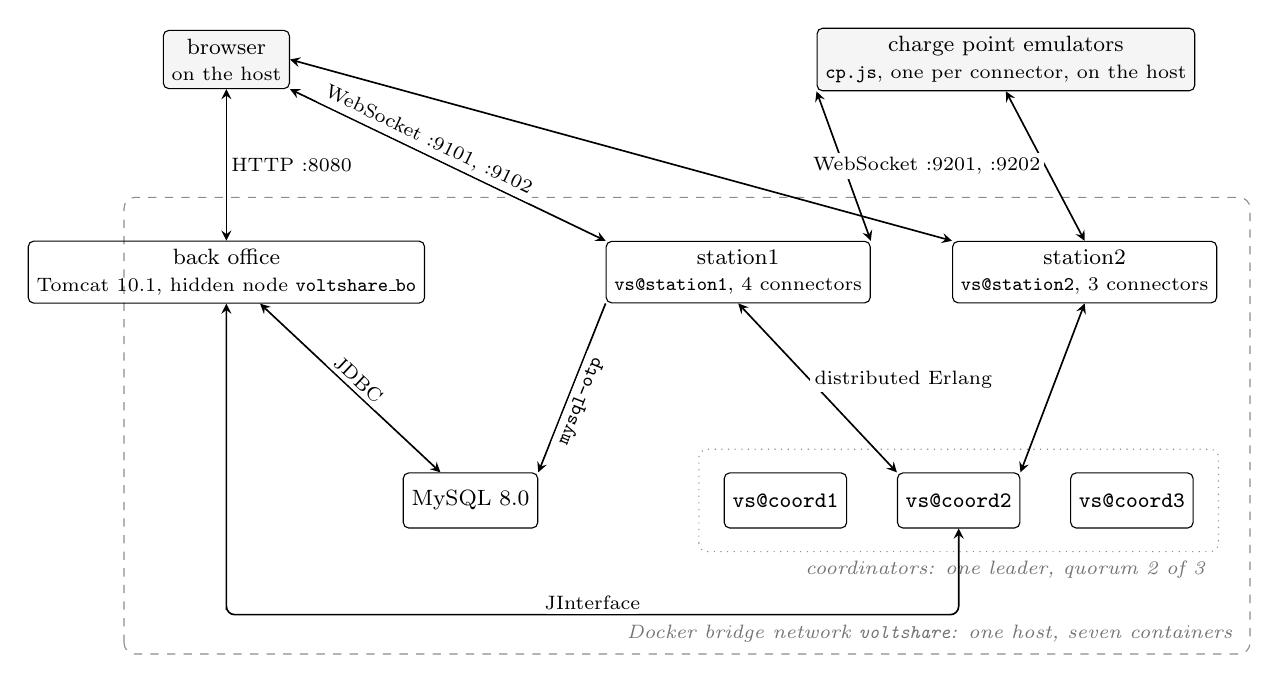
\begin{tikzpicture}[>=stealth, font=\footnotesize, x=1cm, y=1cm,
  nd/.style={draw, rounded corners=2pt, align=center, minimum height=0.7cm, inner sep=3pt},
  host/.style={nd, fill=black!4},
  edge/.style={semithick},
  lab/.style={font=\scriptsize, fill=white, inner sep=1.5pt, align=center}]
  % the one Docker network
  \draw[black!45, dashed, rounded corners=4pt] (1.2,-4.35) rectangle (15.5,1.45);
  \node[font=\scriptsize\itshape, text=black!55, anchor=south east] at (15.4,-4.33)
    {Docker bridge network \texttt{voltshare}: one host, seven containers};
  % nodes
  \node[host] (browser) at (2.5,3.2) {browser\\ \scriptsize on the host};
  \node[host] (emu) at (12.4,3.2) {charge point emulators\\ \scriptsize \texttt{cp.js}, one per connector, on the host};
  \node[nd] (bo) at (2.5,0.5) {back office\\ \scriptsize Tomcat 10.1, hidden node \texttt{voltshare\_bo}};
  \node[nd] (st1) at (9.0,0.5) {station1\\ \scriptsize \texttt{vs@station1}, 4 connectors};
  \node[nd] (st2) at (13.4,0.5) {station2\\ \scriptsize \texttt{vs@station2}, 3 connectors};
  \node[nd] (db) at (5.6,-2.4) {MySQL 8.0};
  \node[nd] (c1) at (9.6,-2.4) {\texttt{vs@coord1}};
  \node[nd] (c2) at (11.8,-2.4) {\texttt{vs@coord2}};
  \node[nd] (c3) at (14.0,-2.4) {\texttt{vs@coord3}};
  \draw[black!45, dotted, rounded corners=3pt] (8.5,-3.05) rectangle (15.1,-1.75);
  \node[font=\scriptsize\itshape, text=black!55, anchor=north east] at (15.05,-3.05)
    {coordinators: one leader, quorum 2 of 3};
  % client-facing edges
  \draw[edge, <->] (browser) -- node[lab, right] {HTTP :8080} (bo);
  \draw[edge, <->] (browser.south east) -- node[lab, above, sloped, pos=0.42] {WebSocket :9101, :9102} (st1.north west);
  \draw[edge, <->] (browser.east) -- (st2.north west);
  \draw[edge, <->] (emu.south west) -- (st1.north east);
  \draw[edge, <->] (emu.south) -- node[lab, left, pos=0.5] {WebSocket :9201, :9202} (st2.north);
  % internal edges
  \draw[edge, <->] (bo) -- node[lab, above, sloped] {JDBC} (db);
  \draw[edge, ->] (st1.south west) -- node[lab, below, sloped, pos=0.55] {\texttt{mysql-otp}} (db.north east);
  \draw[edge, <->] (st1.south) -- node[lab, right, pos=0.45] {distributed Erlang} (c2.north west);
  \draw[edge, <->] (st2.south) -- (c2.north east);
  \draw[edge, <->, rounded corners=3pt] (bo.south) |- (2.5,-3.85) -| node[lab, above, pos=0.25] {JInterface} (c2.south);
\end{tikzpicture}
\caption{The delivered deployment: seven containers on one Docker bridge network, and the
protocol on each edge. Both stations write to MySQL through \texttt{mysql-otp}; one edge is
drawn. The browser and the emulated hardware run on the host and reach the containers
through published ports.}
\label{fig:deployment}
\end{figure}


\paragraph{Back office (Java, Tomcat).} Renders every page server-side and owns everything
durable. It authenticates the driver, mints the JWT that the station will verify on its own,
prices closed sessions, and applies the no-show suspensions. It also joins the Erlang
cluster as a hidden node through JInterface. The leader pushes the station list to it
whenever something visible changes, and at least every 30 seconds.

\paragraph{Coordinator (Erlang/OTP, three instances).} One of them leads and the other two
stand by. The leader grants and refuses claims and keeps the map of which stations are up;
how the other two take over when it goes is \cref{sec:p2b}.

\paragraph{Station (Erlang/OTP with Cowboy, two instances).} Each station runs one
\texttt{gen\_statem} per connector, a manager that arbitrates them and allocates the site
power, and two WebSocket endpoints, one for drivers and one for charge points. The two
stations of the delivered deployment are configured differently:

\begin{itemize}
  \item \texttt{station1}: four connectors rated 150, 150, 150 and 50~kW, on a site budget
        of 350~kW. The demonstration profile lowers that budget to 200~kW so that the
        sharing is visible with two cars.
  \item \texttt{station2}: three connectors rated 150, 50 and 50~kW, on 180~kW.
\end{itemize}

Both sites are oversubscribed like in a real scenario. Four connectors that can draw 500~kW
between them sit behind a 350~kW connection, so the moment three fast chargers are busy the
station has to apportion rather than serve, which is P5 in \cref{sec:p5}.

\paragraph{MySQL.} One instance, holding accounts, vehicles, reservations that completed,
sessions, invoices and notifications. It is a single point of failure for durable data and
we declare it as one in \cref{sec:no-tolerance}.

\paragraph{The browser is not a node.} Pages arrive rendered, and the only state a browser
holds is what its WebSocket has just pushed into the two live views so there is no client-side cache to reconcile after a reconnection, so a page
that comes back gets a complete snapshot and is immediately correct.

\section{Synchronization and Coordination Problems}
\label{sec:problems}

This section states the problems the project set out to solve. The mechanisms that answer
them are in \cref{sec:addressing}, and the ones that answer failures are in
\cref{sec:fault-tolerance}.

Six of them are numbered P1 to P6 and are referred to by those names throughout the
document.

\subsection{The two exclusions in the system}
\label{sec:two-exclusions}

Two resources in this system are exclusive:

\begin{table}[h]
\centering\small
\caption{The two exclusions.}
\label{tab:exclusions}
\begin{tabularx}{\textwidth}{@{}l >{\raggedright\arraybackslash}p{3.2cm}
                               >{\raggedright\arraybackslash}p{4.2cm} X@{}}
\toprule
& Object protected & Contended by & Scope \\
\midrule
P1 & the connector & drivers, among themselves & inside one station \\
P2 & the vehicle & stations, among themselves & across nodes \\
\bottomrule
\end{tabularx}
\end{table}

A connector belongs to exactly one station, so the station decides alone. The vehicle instead, could appear at two stations at the same time, since the driver could open two browser
tabs and presses \emph{reserve} on both, each station finds its own connector free and
grants, and neither can detect the breach, because the fact that would reveal it is held by
neither. The second exclusion is the reason this project has a coordination
problem at all.

\subsection{Problems inside one station}
\label{sec:local-problems}

\paragraph{P1: several drivers want the same connector.} Two requests for connector 3 arrive
in the same millisecond. Both read the connector as free, both proceed, and the outlet ends
up promised twice. This is the classic race on a shared resource, and its solution is
\cref{sec:p1}.

\paragraph{P5: the site cannot power everything at once.} The sum of what the connectors can
deliver exceeds what the site's grid connection can supply, which is true of real
installations and is the reason dynamic load management exists.

A connector
is exclusive and is therefore \emph{granted}. Electrical capacity is divisible and is
therefore \emph{apportioned}, with the apportionment changing every time a car arrives,
leaves, or slows down as its battery fills. See
\cref{sec:p5}.

\subsection{Problems between the client and the system}
\label{sec:client-problems}

\paragraph{P3: somebody stops answering.} A driver reserves a connector and never arrives,
or disappears in the middle of a session with the cable still in the socket. The same problem in a second form: a station holds a claim at the
coordinator and dies, and the coordinator has no way to ask it whether the claim still
matters. See \cref{sec:p3}.

\paragraph{P6: everyone must see the same connector.} Two drivers, the charge point and the
back office all display a connector whose state changes several times a minute. The station
pushes to all of them (\cref{sec:ssr}); what is left to decide is what it pushes. Sending
only the change is smaller, but it leaves a client that misses one message wrong from then
on, with nothing to tell it so. See \cref{sec:p6}.

\subsection{Problems across nodes}
\label{sec:distributed-problems}

\paragraph{P2: one vehicle, one reservation, network-wide.} The scenario of
\cref{sec:two-exclusions}: the same car reserving at two stations at once, with each station
locally correct. See \cref{sec:p2}.

\paragraph{P2b: the authority itself fails.} Once P2 is answered by an authority, that
authority becomes the thing that can fail. If it
crashes, nobody can reserve until something replaces it. If a partition splits the network,
both sides may conclude that the other is gone and each appoint its own authority, and two
authorities granting claims for the same vehicle break exactly the guarantee the authority
exists to provide. "Split brain" is worse than downtime here, because downtime refuses and
split brain grants. See \cref{sec:p2b}.

\paragraph{P4: a station node goes away.} It can crash, or its uplink can be cut.

A crashed node takes its sessions with it: the process metering them is gone and no row
reaches the database. A partitioned node keeps delivering power to the cars plugged into it
while the rest of the network stops hearing from it, so the site works and the operator goes
blind. In both cases the vehicles that station was holding are stranded: their claims are
alive in the coordinator, and their drivers cannot reserve anywhere else until those claims
expire. See \cref{sec:station-failures}.

\section{Architecture Protocols}
\label{sec:protocols}

\Cref{tab:edges} maps the edges of the system; the middleware choices are argued in
\cref{sec:why-middleware} and the messages are specified in \cref{sec:api}. What this
section adds is which party opens each connection, which way authority flows, and what was
kept off an edge.

\begin{table}[h]
\centering\small
\renewcommand{\arraystretch}{1.15}
\caption{The edges of the system. ``Opened by'' is the side that dials.}
\label{tab:edges}
\begin{tabularx}{\textwidth}{@{}l l l X@{}}
\toprule
Edge & Protocol & Opened by & Carries \\
\midrule
\multicolumn{4}{@{}l}{\emph{Client-facing}} \\
browser $\leftrightarrow$ back office & HTTP & browser & forms and server-rendered pages;
  login session in \texttt{HttpSession} \\
browser $\leftrightarrow$ station & WebSocket, JSON & browser & reserve, cancel, stop; the
  station snapshot and the live session, pushed \\
charge point $\leftrightarrow$ station & WebSocket, JSON & charge point & cable and meter
  reports up, power limits and stop commands down; reduced OCPP 1.6-J \\
\midrule
\multicolumn{4}{@{}l}{\emph{Internal}} \\
station $\leftrightarrow$ coordinator & distributed Erlang & station & claims, renewals,
  announcements, statistics; node monitoring in both directions \\
back office $\leftrightarrow$ coordinator & JInterface & back office & the station
  directory and the leader, pushed; suspensions, pushed back \\
station, back office $\to$ MySQL & SQL & each & one \texttt{INSERT} per closed session
  from the station (\texttt{mysql-otp}); everything else from Java (JDBC) \\
\bottomrule
\end{tabularx}
\end{table}

\subsection{Client-facing edges}
\label{sec:protocols-client}

The browser talks to two servers, and that is the first decision on this map. Pages come
from the back office over HTTP, rendered by servlets and JSP (\cref{sec:ssr}); everything
that happens at a station, reserving, watching a charge, stopping it, goes over a WebSocket
opened \emph{directly to the station node}. The alternative was to route driver traffic
through Tomcat, which would have kept one origin and one authentication scheme. We rejected
it because it puts the web tier on the path of every reservation and every live frame: a
Tomcat restart would have blanked every charging page in the network, and the station could
no longer keep a site working while the back office is down. The price is a second
authentication: the back office mints a JWT, the station verifies it locally and never
calls back (\cref{sec:api-jwt}).

The charge point has an edge of its own, kept apart from the driver's. One party asks and
the other reports; matching a reported cable against a reservation is the station's job.
The charge point dials the station, one socket per connector, as real equipment dials an
operator's backend from behind a site network; the station never dials hardware
(\cref{sec:api-ws-cp}).

\subsection{Internal edges}
\label{sec:protocols-internal}

Between Erlang nodes the protocol is distributed Erlang, with registered names on both
sides so that nobody holds an address, and the same connection carries \texttt{nodedown}
(\cref{sec:detectors}). Stations call, the coordinator answers. It is never on the path of
a charge, which is what lets a coordination outage cost only new reservations
(\cref{sec:api-claim}).

The back office joins the cluster as a hidden Erlang node through JInterface: it receives
the directory and the leader as they change and pushes suspensions back, and no page ever
asks the cluster a question at request time (\cref{sec:api-bridge}). Being hidden, it takes
no part in the quorum: the web tier must never influence who leads.

MySQL is reached from two runtimes, and the rule that makes that safe is written at the top
of \texttt{schema.sql}: \textbf{one writer per table}. The station writes one row, the
closed session, through \texttt{mysql-otp}; Java owns the other tables and the cost of a
session after the fact. The no-show counter is written by Java alone, from a report the
station sends through the coordinator: a counter incremented from several nodes would have
been a second contended object.

What is kept off the internal edges is as telling as what travels on them: no replicated
log between the coordinators (\cref{sec:rebuild}), and no station talking to another.

\section{Addressing the Problems}
\label{sec:addressing}

\Cref{sec:problems} listed the problems. This section describes the mechanism
chosen for each one, the alternatives that were set aside, and what each choice
costs.

\subsection{Mutual exclusion on a connector (P1)}
\label{sec:p1}

Each physical connector is owned by one Erlang process, a \texttt{gen\_statem}
implemented in \texttt{vs\_connector}. Every request that touches that outlet
becomes a message in that process's mailbox, and messages are handled one at a
time, so two drivers reserving the same connector in the same millisecond are
serialised by the runtime and the second finds it already \texttt{held}.

\paragraph{Which driver wins.} Since Erlang guarantees FIFO order point to point
and nothing across senders, the connector goes to the driver whose message the
runtime delivers first. Mutual exclusion is the property claimed here, and nothing
in this domain asks for more.

The machine gives a second guarantee: with the wrong vehicle, \texttt{charging} is
unreachable from \texttt{held}, so no session can start on a connector somebody
else holds. The transition does not exist, so there is no check to forget.

\subsection{One reservation per vehicle, network-wide (P2)}
\label{sec:p2}

The mechanism adopted is a
\emph{claim}: a permission, granted by the coordinator, recording that a given
vehicle is now committed and to which station.

\subsubsection{Claim first, commit after}

A station obtains the claim \emph{before} it creates the reservation.

In the wrong order, a crash between the two steps leaves a reservation that no
other node knows about, allowing the vehicle can then obtain a second reservation
elsewhere. In the right order, the same crash leaves a claim that was granted and
never used. Nobody can reserve for that vehicle for a few minutes, and then the
claim expires on its own. The system errs towards refusing rather than towards
granting twice.

\subsubsection{Why a central arbiter}

The coordinator is a single process, \texttt{vs\_coord\_srv}, and its claim table
is a map keyed by vehicle. Requests from different stations queue in its mailbox
and are decided one at a time. This is the centralised mutual exclusion where there is one critical section per vehicle. Two claims for two different cars
contend over nothing, and what the mailbox serialises is the instant of the
decision.

Three designs were considered.

\paragraph{One coordinator, unreplicated.} The simplest, and it leaves an
avoidable single point of failure.

\paragraph{A \texttt{UNIQUE} constraint in MySQL.} Correct, and almost free to
write. But the coordinator has to exist anyway for the cluster map and for node
monitoring, so this removes no component, and a claim that \emph{expires by
itself} is a timer inside a process, while in a database it becomes a cleanup job
or a filter on every read.

\paragraph{Direct coordination between stations (Ricart-Agrawala).} No central
authority, at $2(n-1)$ messages per reservation, and it serialises access to
\emph{one} critical section: here two reservations for two different vehicles
would wait for each other with nothing to gain.

What we built is the first one with its single point of failure removed: one
arbiter serving at a time, elected among three coordinator nodes and required to
hold a quorum, which is \cref{sec:p2b}.

\subsubsection{Ordering decided by one clock}

When a claim is granted, the coordinator stamps it with \texttt{granted\_at} and
sends that timestamp back with the grant. The station stores it and echoes it in
the renewal it sends every ten seconds for all the claims it holds
(\cref{sec:p3}).

The purpose is conflict resolution after a failover. If two claims for the same
vehicle ever meet in the table, the older one wins, and the comparison is between
two timestamps produced by the \emph{same} process. No two machines with
unsynchronised clocks are ever compared.

\subsection{Leases (P3)}
\label{sec:p3}

The problem of the driver who reserves and never arrives is approached by a lease: every reservation is granted with an expiry, and
when it passes the connector returns to \texttt{free} with no operator action and
no cooperation from the party that disappeared.

There are two nested expiries, and they protect against two different absent
parties:

\begin{itemize}
  \item the \textbf{reservation lease} protects against the driver who never
        shows up. It is the timer the connector process holds;
  \item the \textbf{claim expiry} protects against the station that dies without
        releasing what it holds. A renewal keeps the claim alive, so a station
        that crashes stops renewing and its claims expire on their own.
\end{itemize}


\subsection{Coordinator replication: election and quorum (P2b)}
\label{sec:p2b}

Three coordinator nodes run, \texttt{vs@coord1}, \texttt{vs@coord2} and
\texttt{vs@coord3}, and every node of the cluster is configured with the same
three names. One of them is the leader and is the only node that grants or refuses
claims. A station that addresses one of the other two is redirected to the leader.

\paragraph{Election.} When the leader stops responding, the survivors elect a new
one with the bully algorithm over those names: the list is sorted, and the highest
live entry wins, so a cluster in good health is led by \texttt{vs@coord3}. A node that notices the leader is gone sends \texttt{ELECTION}
to the nodes above it. Silence means it is the most senior node alive and it
announces \texttt{LEADER} downwards; an answer means somebody more senior is
handling it, and it waits. With three nodes this settles in two rounds of
messages. Detection is by timeout, which means we assume a \emph{synchronous}
system, an upper bound on response time.

\paragraph{Quorum.} Bully alone does not prevent split brain. In a partition each
side happily elects its own local maximum, and two authorities granting claims
break precisely the invariant the coordinator exists to protect. So a coordinator
serves only while it can see a majority of the configured coordinator cluster,
itself included: two out of three. A node in the minority suspends itself and
refuses everything, leader or not.

This is why the cluster has three members and not two. With an even number, a
partition can produce two halves that each consider themselves entitled to grant.

\paragraph{State after a failover.} Since a new leader inherits nothing, it asks the stations what they hold and
rebuilds the claim table from their answers. The reason of this approach is developed in
\cref{sec:rebuild}.

\subsection{Sharing the site power (P5)}
\label{sec:p5}

An Erlang module, \texttt{vs\_power}, recomputes the split on every arrival and departure, and on a
periodic tick that follows the charging curve as batteries fill.

The policy is max-min fair share with hand-back. Every active session starts from
$budget/N$. A session that cannot absorb its share, either because the car is
small or because it is tapering near full, takes only what it asks for and hands
the surplus back, which is then split again among the others. The loop repeats
until nobody hands anything back or the budget is exhausted.


\subsection{One source of truth for every client (P6)}
\label{sec:p6}

The cheapest way to make every client agree is to give them nothing to compute.
The station holds the authoritative state and pushes a \emph{complete} snapshot of
it, so that each page that misses a
message is wrong only until the next push, and one that reconnects is correct
immediately. Snapshots go out on every change and on a periodic tick.


\section{Fault Tolerance and Recovery}
\label{sec:fault-tolerance}

Fault tolerance in this system relies on five mechanisms selected based on the type of fault.

\subsection{The failure model}
\label{sec:failure-model}

We assume crash-stop and network partition. Byzantine behaviour is out of scope. \Cref{tab:failures} lists what can fail
and what the system does about it.

\begin{table}[t]
\centering\small
\renewcommand{\arraystretch}{1.2}
\caption{What can fail, how it is noticed, and what it costs.}
\label{tab:failures}
\begin{tabularx}{\textwidth}{@{}>{\raggedright\arraybackslash}p{2.6cm}
                               >{\raggedright\arraybackslash}p{2.9cm}
                               X
                               >{\raggedright\arraybackslash}p{2.9cm}@{}}
\toprule
What fails & How it is noticed & What happens & What is lost \\
\midrule
Coordinator, crash & \texttt{nodedown}, at once &
  election; the new leader rebuilds from the stations &
  nothing \\
Coordinator, partition & heartbeat, 3~s &
  the minority suspends itself &
  new reservations, minority side \\
Station node, crash & \texttt{monitor\_node}, at once &
  the coordinator drops that station's claims &
  sessions running there \\
Station uplink, partition & \texttt{monitor\_node}, on the tick &
  the site keeps charging, starts nothing new &
  the operator's view \\
Charge point & socket closes, then 30~s grace &
  session closed with the last measured energy &
  nothing measured \\
Back office & nothing, it is a hidden node &
  the cluster is unaffected; it re-reads on restart &
  nothing durable \\
MySQL & connection errors &
  not tolerated, see \cref{sec:no-tolerance} &
  writes, until it returns \\
\bottomrule
\end{tabularx}
\end{table}

\subsection{Two failure detectors, because there are two failures}
\label{sec:detectors}

\texttt{net\_kernel:monitor\_nodes/1} comes for free and fires the instant a TCP
connection breaks, which is what a killed container looks like. A partition breaks
nothing: the peer is unreachable but its socket stays open, so no
\texttt{nodedown} is delivered until the distribution's own tick expires, and
\texttt{net\_ticktime} defaults to sixty seconds. A minority leader would go on
granting claims for a minute without knowing it had lost its quorum.

Liveness is therefore decided by a heartbeat among the coordinators, implemented
in \texttt{vs\_coord\_membership}: each announces itself once a second, and three
missed announcements mean gone. Three seconds instead of sixty. It runs among the
three coordinators only, because that is where a stale view produces two leaders;
a station that goes silent is still noticed on the tick, at the cost
\cref{tab:failures} states. \texttt{monitor\_nodes} stays subscribed for the crash
case, where it is faster still.

Measured on 1 September, isolating the leader with
\texttt{docker network disconnect}:

\begin{itemize}
  \item \texttt{QUORUM LOST (1 of 3) \ldots{} abdicating} at \textbf{2.12~s};
  \item a new leader serving with both claims at \textbf{2.29~s};
  \item the distribution's own \texttt{nodedown} at \textbf{64.6~s}.
\end{itemize}

That last number is the argument. Without the heartbeat the system would have
been incorrect for a full minute, and no test would have revealed it, because
\texttt{docker kill}, the obvious way to simulate a failure, closes the socket
and never exercises this path at all. Two kinds of failure need two experiments,
which is why the demonstration shows both \texttt{kill} and \texttt{disconnect}.

\subsection{A station dies}
\label{sec:station-failures}

\texttt{vs\_coord\_srv} monitors every station it has
heard from and, on \texttt{nodedown}, erases that station's claims. Keeping them
would shut those drivers out of the whole network until the lease expired.

The cars carry on charging, because the node is not on the path that delivers
power. The charge point is also the side that counts the energy, so when the
station comes back it reports its running total, the station adopts the session
from it, and the charge is billed in full. What is lost is a car that unplugs
while the node is still down: nothing writes its row, and that energy is never
invoiced.

\subsection{Rebuilding the claim table after a failover}
\label{sec:rebuild}

The new leader must discover the claims by querying the system.
It sends a \texttt{who\_do\_you\_hold} message to each station; the station examines its connectors and responds by indicating those in the \texttt{held} (occupied) or \texttt{charging} state, based on its local memory.
The leader transitions from the \texttt{rebuilding} state to the \texttt{serving} (operational) state once the responses are received.
Requests received in the interim are rejected with a retry indication, which the stations interpret as a temporary refusal.

\paragraph{Convergence via two paths.} 
The system would converge autonomously without the need for explicit queries from the new coordinator, as stations renew their claims every 10 seconds;
however, the query allows for a significant reduction in recovery time.

\subsection{A charge point dies}
\label{sec:cp-failure}

A lost socket is not a broken charger, so the connector waits ninety seconds
before doing anything: sixty of socket idle timeout, thirty of its own grace. If
they run out mid-session, the session is closed with the last energy the charge
point reported, the only figure anybody measured, and the connector goes
\texttt{out\_of\_service} until a charge point boots and reports itself available.

\subsection{Supervision inside a node}
\label{sec:supervision}


Three supervisory strategies have been implemented:

\begin{lstlisting}[caption={The two supervision trees. The station nests a second
                   supervisor inside the first; the coordinator does not.},
                   label={lst:suptrees}]
vs_station_sup                      one_for_one
  +-- vs_connector_sup              simple_one_for_one
  |     +-- vs_connector            connector 1   started at boot by
  |     +-- vs_connector            connector 2   vs_station_mgr, one
  |     +-- vs_connector            connector N   per physical connector
  +-- vs_station_mgr
  +-- vs_claim_client
  +-- vs_station_db

vs_coord_sup                        rest_for_one
  +-- vs_coord_srv                  claim table, cluster map
  +-- vs_coord_bo                   JInterface bridge to the back office
  +-- vs_coord_election             bully election
  +-- vs_coord_membership           heartbeat and quorum
      declaration order is dependency order
\end{lstlisting}

A supervisor restarts its children, and the strategy decides which ones go down
together. The two trees choose differently.

The coordinator is \texttt{rest\_for\_one}: its children are declared in
dependency order, so a process that dies takes with it everyone declared after
it. The bridge publishes what the claim table holds, and must not outlive a table
that was restarted underneath it.

The station is \texttt{one\_for\_one}: its children are independent and restart
alone. Connectors find the manager by registered name and hold no reference to
it, so a manager that comes back re-adopts them and no session is lost. The
connectors are all the same kind of process, one per outlet, hence
\texttt{simple\_one\_for\_one}; one that crashes comes back in \texttt{free}.

\subsection{Delivery semantics, chosen per message}
\label{sec:guarantees}

The bridge from the coordinator to the back office carries three kinds of event,
and they deliberately do not get the same guarantee, because the cost of a
duplicate is different for each.

\begin{itemize}
  \item \textbf{The session row: at-least-once over an idempotent write.} The
        message itself is never resent. What makes it at-least-once is that the
        station has already written the row at the end of the session, and the
        back office sweeps \texttt{cost\_cents IS NULL} every sixty seconds, so
        the event only makes an invoice arrive sooner and losing it costs one
        interval. The price is written with \texttt{UPDATE sessions SET
        cost\_cents = ? WHERE id = ? AND cost\_cents IS NULL}: a repeat updates
        zero rows, which is not an error.
  \item \textbf{The no-show strike: maybe.} One send, no retransmission and no
        duplicate filter. A counter cannot recognise a duplicate, so a retry
        could suspend an innocent driver, and a lost strike is a smaller wrong
        than an invented one.
  \item \textbf{The notification to the driver: maybe}, for the same reason. A duplicate is a
        row somebody reads twice, a loss is a row they never see, and we chose
        the quieter failure.
\end{itemize}

\subsection{What tolerates nothing, and is declared}
\label{sec:no-tolerance}

Three things here have no recovery path.

\textbf{MySQL is a single point of failure} for durable data. Replicating it was
out of reach for this project. This choice leads some limitations:

\textbf{Sessions on a dead station are lost}, as \cref{sec:station-failures}
describes. The process that was metering them is gone.

\textbf{The rebuild can still miss a station that is unreachable at exactly the
wrong moment.} Its claims are absent from the new leader's table, so one of its
vehicles could obtain a second claim before the conflict is noticed. The window
is narrow and it is real, and it closes when the station returns and re-presents
the older claim, which wins.

\section{API and Protocol Specification}
\label{sec:api}

Five channels carry everything in this system, and \cref{sec:protocols} said which runs where
and why. This section specifies what travels on each one.

\subsection{HTTP: browser to back office}
\label{sec:api-http}

Nine servlets, mapped with \texttt{@WebServlet} annotations.
Everything is rendered server-side and forwarded to a JSP; there is no JSON API on this
channel, because the browser receives pages.

\begin{table}[h]
\centering\small
\renewcommand{\arraystretch}{1.15}
\caption{HTTP endpoints of the back office. The last column marks the ones behind
\texttt{AuthFilter}.}
\label{tab:http}
\begin{tabularx}{\textwidth}{@{}l l X c@{}}
\toprule
Path & Method & Effect & Auth \\
\midrule
\texttt{/register} & POST & creates the account and its vehicle profile & \\
\texttt{/login} & POST & authenticates, opens the \texttt{HttpSession}, mints the JWT & \\
\texttt{/logout} & GET & invalidates the session & \\
\texttt{/stations} & GET & the directory, read from \texttt{StationDirectory} in memory &
  $\bullet$ \\
\texttt{/station} & GET & one station's page, with the JWT and the WebSocket URL &
  $\bullet$ \\
\texttt{/session} & GET & the live session page for a connector & $\bullet$ \\
\texttt{/profile} & GET & account and vehicle & $\bullet$ \\
\texttt{/history} & GET & past sessions with their invoices & $\bullet$ \\
\texttt{/notifications} & GET & notifications stored for this driver & $\bullet$ \\
\bottomrule
\end{tabularx}
\end{table}

\subsubsection{The token the station will trust}
\label{sec:api-jwt}

A station has to recognise a driver without asking the back office, which is what keeps a
site working while Tomcat is down. The token is the only thing the two sides share.

It is a JWT signed with \textbf{HS256} using a symmetric secret, passed to both sides in the
environment as \texttt{VOLTSHARE\_JWT\_SECRET}. It lives 60 minutes. Java signs with \texttt{jjwt},
Erlang verifies with \texttt{jose}.

\begin{lstlisting}[language=json, caption={The claims, plus the standard \texttt{iat}.},
                   label={lst:jwt}]
{ "sub": "12", "username": "andrea", "vehicle_id": 88,
  "iss": "voltshare-backoffice", "exp": 1755792000 }
\end{lstlisting}

\texttt{sub} is the user id as a string, which the JWT specification requires, and
\texttt{vehicle\_id} is a number. The station needs both: the first attributes the session
to an account, the second matches the claim, which is per vehicle.

On the first frame of the WebSocket the station verifies the signature, checks that \texttt{iss} is exactly
\texttt{voltshare-backoffice}, checks that \texttt{exp} is in the future, and extracts the
two identifiers. A failure closes the socket with \texttt{4401}, an expired token with
\texttt{4408}. The station never calls the back office about a token, whether it accepts one
or throws it out.

There is a trap here that the library invites, and \texttt{contracts/sample-tokens.md}
records it: \texttt{jose\_jwt:verify/2} checks \emph{only the signature}. Issuer and expiry
are ordinary claims, so a token that verifies is not yet a token to accept, and both checks
are written out explicitly on the station side.

\paragraph{How the token reaches the browser.} The servlet puts it in the session, the JSP
renders it into a hidden \texttt{data-} attribute through \texttt{<c:out>}, and the
WebSocket code reads it from there. 

\subsection{WebSocket: driver to station}
\label{sec:api-ws-driver}

The page opens \texttt{ws://<station>:8080/ws/driver?station\_id=<id>}. Host and port are
what the station announced about itself, republished by \texttt{StationDirectory}
(\cref{sec:api-bridge}). The page appends the query string, naming the station it believes
it is showing. A mismatch closes the socket with \texttt{4400}.

Frames are text, one JSON object each, and both directions share one envelope.

\begin{lstlisting}[language=json, label={lst:envelope},
  caption={The envelope of both WebSocket channels. A \texttt{payload} is \texttt{\{\}} when
  there is nothing to say.}]
// browser -> station
{ "action": "reserve", "request_id": "3f2c9a",
  "payload": { "connector_id": 3 } }

// station -> browser
{ "type": "ack", "request_id": "3f2c9a",
  "payload": { "expires_at": 1757250000000, "lease_seconds": 900 } }
\end{lstlisting}

Every decision is taken in \texttt{vs\_driver\_proto}, a module of pure functions over a
session map, so the whole contract runs under EUnit with no listener.
\texttt{vs\_driver\_ws} holds the Cowboy callbacks and nothing else. The rest of this
subsection walks the channel in the order the frames occur, with the real shape of each one.

\paragraph{Join, and nothing before it.} The socket starts unauthenticated, and the first
frame has to be a \texttt{join} carrying the JWT of \cref{sec:api-jwt}, within 5~s.

\begin{lstlisting}[style=msg]
{ "action": "join", "request_id": "r-join",
  "payload": { "token": "eyJhbGciOiJIUzI1NiJ9.eyJzdWIiOiIxMiIs...<sig>" } }
\end{lstlisting}

\texttt{token} is the only field read. The station verifies it locally and binds
\texttt{user\_id} and \texttt{vehicle\_id} to the connection, so a payload that also carries
a \texttt{user\_id} changes nothing. The answer is an empty \texttt{ack}, with the first
\texttt{state} behind it in the same write.

\begin{lstlisting}[style=msg]
{ "type": "ack", "request_id": "r-join", "payload": {} }
\end{lstlisting}

\paragraph{Reserve, cancel, stop.} Three actions follow, and every one names a connector.

\begin{lstlisting}[style=msg]
{ "action": "reserve", "request_id": "a1", "payload": { "connector_id": 3 } }
\end{lstlisting}

The station asks the coordinator for a claim before it touches the connector
(\cref{sec:api-claim}). Only if the claim is granted does the connector go \texttt{held},
and the \texttt{ack} carries the lease that the page counts down from.

\begin{lstlisting}[style=msg]
{ "type": "ack", "request_id": "a1",
  "payload": { "connector_id": 3,
               "expires_at": 1757250000000, "lease_seconds": 900 } }
\end{lstlisting}

\texttt{expires\_at} is epoch milliseconds and \texttt{lease\_seconds} is the same lease as a
duration, both from the station's clock. A refusal arrives instead, echoing the same
\texttt{request\_id} and carrying a code from \cref{tab:driver-errors}.

\begin{lstlisting}[style=msg]
{ "type": "error", "request_id": "a1",
  "payload": { "code": "ALREADY_HELD",
               "message": "connector 3 is held by another driver" } }
\end{lstlisting}

\texttt{cancel\_reservation} and \texttt{stop\_session} carry the payload of
\texttt{reserve} and are acknowledged with the connector alone,
\texttt{"payload": \{ "connector\_id": 3 \}}. Cancelling frees the connector at once and
releases the claim, with no penalty, which is the whole incentive to cancel. Stopping tells
the charge point to stop and returns the connector's share to the pool, while the session
row waits for the vehicle to be unplugged.

\Cref{fig:seq-reserve} puts these frames on a timeline, with a lost \texttt{ack} and a
second reservation for the same vehicle.

\begin{figure}[t]
\centering
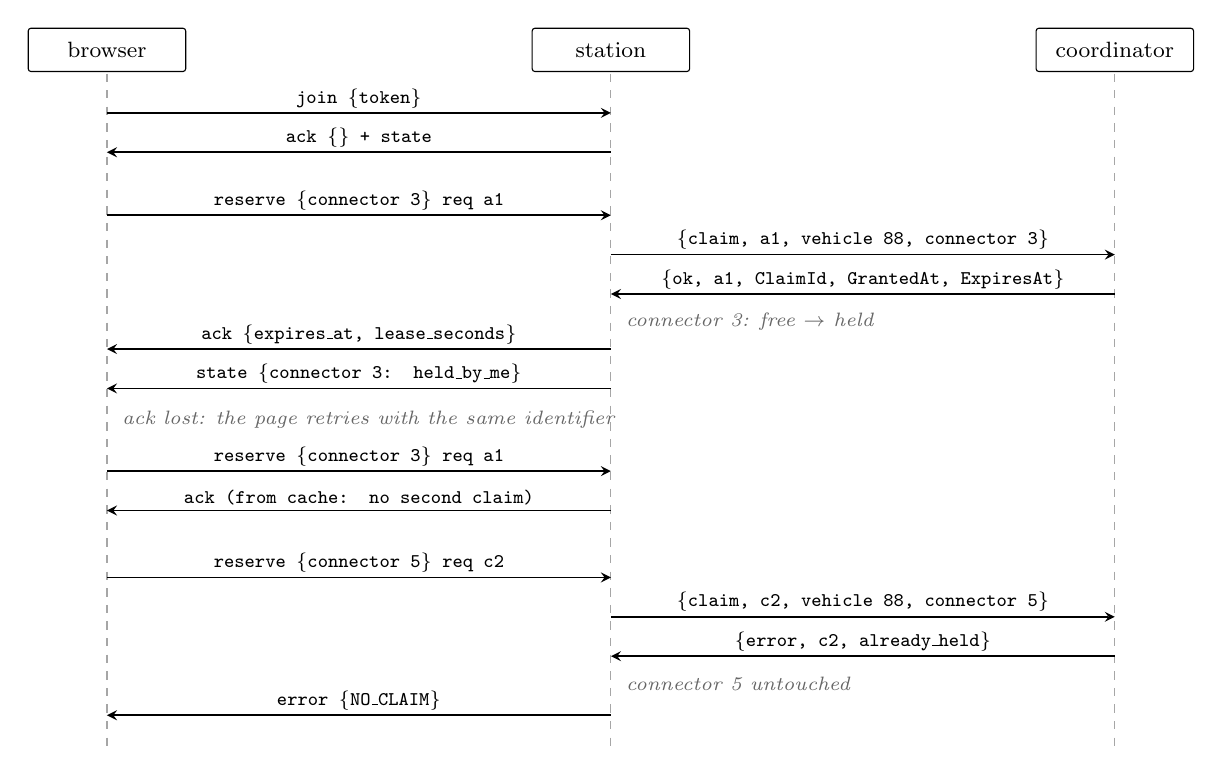
\begin{tikzpicture}[>=stealth, font=\footnotesize, x=1cm, y=1cm,
  msg/.style={->, semithick},
  lab/.style={font=\scriptsize\ttfamily, fill=white, inner sep=1.5pt, midway},
  note/.style={font=\scriptsize\itshape, text=black!60, anchor=west, inner sep=1pt}]
  \foreach \x/\n in {0/browser, 6.4/station, 12.8/coordinator} {
    \node[draw, rounded corners=1pt, minimum width=2cm, minimum height=0.55cm] at (\x,0) {\n};
    \draw[black!35, dashed] (\x,-0.3) -- (\x,-8.9);
  }
  \draw[msg] (0,-0.8) -- (6.4,-0.8) node[lab, above] {join \{token\}};
  \draw[msg] (6.4,-1.3) -- (0,-1.3) node[lab, above] {ack \{\} + state};
  \draw[msg] (0,-2.1) -- (6.4,-2.1) node[lab, above] {reserve \{connector 3\}  req a1};
  \draw[msg] (6.4,-2.6) -- (12.8,-2.6) node[lab, above] {\{claim, a1, vehicle 88, connector 3\}};
  \draw[msg] (12.8,-3.1) -- (6.4,-3.1) node[lab, above] {\{ok, a1, ClaimId, GrantedAt, ExpiresAt\}};
  \node[note] at (6.55,-3.45) {connector 3: free $\rightarrow$ held};
  \draw[msg] (6.4,-3.8) -- (0,-3.8) node[lab, above] {ack \{expires\_at, lease\_seconds\}};
  \draw[msg] (6.4,-4.3) -- (0,-4.3) node[lab, above] {state \{connector 3: held\_by\_me\}};
  \node[note] at (0.15,-4.7) {ack lost: the page retries with the same identifier};
  \draw[msg] (0,-5.35) -- (6.4,-5.35) node[lab, above] {reserve \{connector 3\}  req a1};
  \draw[msg] (6.4,-5.85) -- (0,-5.85) node[lab, above] {ack (from cache: no second claim)};
  \draw[msg] (0,-6.7) -- (6.4,-6.7) node[lab, above] {reserve \{connector 5\}  req c2};
  \draw[msg] (6.4,-7.2) -- (12.8,-7.2) node[lab, above] {\{claim, c2, vehicle 88, connector 5\}};
  \draw[msg] (12.8,-7.7) -- (6.4,-7.7) node[lab, above] {\{error, c2, already\_held\}};
  \node[note] at (6.55,-8.05) {connector 5 untouched};
  \draw[msg] (6.4,-8.45) -- (0,-8.45) node[lab, above] {error \{NO\_CLAIM\}};
\end{tikzpicture}
\caption{A reservation on the driver channel: the claim precedes the commit, a retried
\texttt{reserve} is answered from the cache, and a second reservation for the same vehicle
is refused by the coordinator before the station touches the connector.}
\label{fig:seq-reserve}
\end{figure}

\paragraph{What the station pushes.} \texttt{ack} and \texttt{error} answer an action and
echo its \texttt{request\_id}. The other three arrive unasked and carry \texttt{null} there.
\texttt{state} is the whole station, sent on join, on every change, and every 5~s.

\begin{lstlisting}[style=msg]
{ "type": "state", "request_id": null,
  "payload": {
    "station_id": 1, "name": "Pisa Centro",
    "site_power_kw": 350, "allocated_kw": 210.5, "tariff_cents_kwh": 45,
    "coordinator_reachable": true,
    "connectors": [
      { "connector_id": 2, "state": "held", "rated_kw": 150, "power_kw": 0,
        "held_by_me": true, "mine": true, "expires_at": 1757250000000 },
      { "connector_id": 3, "state": "charging", "rated_kw": 150,
        "held_by_me": false, "mine": false, "expires_at": null,
        "power_kw": 120.0 } ],
    "waitlist": { "length": 0, "my_position": null } } }
\end{lstlisting}

A connector's \texttt{state} is one of \texttt{free}, \texttt{held}, \texttt{charging},
\texttt{suspended}, \texttt{complete}, \texttt{overstay}, \texttt{closing} and
\texttt{out\_of\_service}, the last being the wire name for a connector with no process
answering for it. \texttt{held\_by\_me} and \texttt{mine} are not synonyms: the first means
the reservation belongs to this driver, the second also covers a session in progress. The
\texttt{waitlist} object is a constant, left in place for the feature of \cref{sec:future}.
The periodic tick earns its place beside the event-driven pushes, because meter readings
change \texttt{power\_kw} without raising a connector event, and an event-only channel would
show a live session at a frozen power. A WebSocket \texttt{ping} rides on the same tick, so
that Cowboy's inbound-only idle timeout does not hang up on a page that is only watching.

\texttt{session} goes out with each \texttt{state}, and only to the owner of a running
session. A driver without one gets no frame at all, instead of a frame of zeros.

\begin{lstlisting}[style=msg]
{ "type": "session", "request_id": null,
  "payload": { "connector_id": 2, "phase": "charging",
               "power_kw": 89.4, "energy_kwh": 12.317, "soc_pct": 58,
               "eta_seconds": 981, "started_at": 1757248000000,
               "overstay_seconds": 0 } }
\end{lstlisting}

\texttt{phase} is \texttt{charging}, \texttt{suspended}, \texttt{complete},
\texttt{overstay} or \texttt{closed}, read off the connector in that order of precedence, so
that a car which is both full and past its grace period reports \texttt{overstay}.
\texttt{eta\_seconds} is \texttt{null} while nothing is being delivered.
\texttt{overstay\_seconds} is already net of the grace, and it is the same number that ends
up in \texttt{sessions.\allowbreak overstay\_seconds}. A session ends by disappearing from
the snapshot, and that disappearance becomes one last frame with the phase \texttt{closed}.

\begin{lstlisting}[style=msg]
{ "type": "notification", "request_id": null,
  "payload": { "kind": "reservation_expiring", "connector_id": 3,
      "text": "Your reservation expires in less than two minutes." } }
\end{lstlisting}

There are six kinds: \texttt{reservation\_expiring}, \texttt{reservation\_expired},
\texttt{claim\_revoked}, \texttt{charge\_complete}, \texttt{overstay\_started} and
\texttt{session\_interrupted}. The manager broadcasts each event to every subscribed socket,
and a socket delivers it only when the user it names is the user its token bound. One table
supplies the sentence for this frame and for the durable copy that reaches
\texttt{notifications.jsp}, so both say the same words.

\paragraph{Two ways for something to go wrong.} A refused action produces an \texttt{error}
frame and leaves the connection open. \Cref{tab:driver-errors} is the whole set of nine
codes, and a driver waiting on a reservation always gets one of them or an \texttt{ack}.

\begin{table}[h]
\centering\small
\renewcommand{\arraystretch}{1.15}
\caption{The nine application error codes, carried in the \texttt{code} field of an
\texttt{error} frame. The \texttt{message} beside them is written for the driver and the
page shows it verbatim.}
\label{tab:driver-errors}
\begin{tabularx}{\textwidth}{@{}l X@{}}
\toprule
Code & Raised when \\
\midrule
\texttt{BAD\_REQUEST} & the frame is unusable: no \texttt{request\_id}, no \texttt{payload}
  object, an unknown action, or a \texttt{connector\_id} that is not a positive integer \\
\texttt{UNAUTHENTICATED} & an action arrived before \texttt{join} succeeded, and the socket
  is then closed with \texttt{4401} \\
\texttt{UNKNOWN\_CONNECTOR} & that connector is not one of this station's \\
\texttt{RETRY\_LATER} & the condition is temporary: the coordinator is rebuilding, the
  station is starting, or the connector process is between a crash and its restart \\
\texttt{ALREADY\_HELD} & another driver holds that connector \\
\texttt{NO\_CLAIM} & the vehicle already holds a reservation, or the coordinator never
  answered \\
\texttt{SUSPENDED} & the account is serving a no-show penalty, and walk-in charging still
  works \\
\texttt{NOT\_YOURS} & that reservation or session belongs to another account \\
\texttt{INVALID\_STATE} & the action does not apply to the connector as it is now \\
\bottomrule
\end{tabularx}
\end{table}

A close code is the other kind, and it ends the connection. \texttt{4400} covers a binary
frame, malformed JSON or a wrong \texttt{station\_id}. \texttt{4401} covers a bad token, an
action before \texttt{join}, or no \texttt{join} within the 5~s. \texttt{4408} is an expired
token, kept apart so that the page can tell ``log in again'' from ``something is wrong''.
\texttt{1001} is the station shutting down. The page treats the first three as final and
answers the last by reconnecting with backoff.

\paragraph{Decisions on this channel.}
\begin{itemize}
  \item \textbf{Identity comes from the token alone.} \texttt{held\_by\_me}
        and \texttt{mine} are computed on the station. A notification is delivered only when
        the user it names is the one the token bound, a filter written as a pattern in the
        clause head of \texttt{websocket\_info/2}. The alternative was a \texttt{user\_id}
        field in the request. It would let a driver reserve or cancel for somebody else by
        editing a frame.
  \item \textbf{One \texttt{RETRY\_LATER}, with the cause in the message.} Three facts share
        the code: the coordinator is rebuilding, the station is starting, or the connector
        process is between a crash and its restart. The client does the same thing in all
        three. Three codes would put a piece of the station's internals into every client.
        The third case used to be answered \texttt{UNKNOWN\_CONNECTOR}, a permanent code for
        a condition that lasts milliseconds.
  \item \textbf{The socket keeps no state; the connector process does.} Reconnection is the
        client's job: backoff from 500~ms, capped at 10~s, then a fresh \texttt{join}. The
        station keeps nothing for a disconnected socket. The reservation lives in the
        connector process and survives the browser being closed.
\end{itemize}

\subsection{WebSocket: charge point to station}
\label{sec:api-ws-cp}

This channel is the boundary of the system. Above it is production logic, below it is
emulated hardware. The emulator is credible only if a real charge point could implement the
same interface. The message set is a reduced OCPP 1.6-J~\cite{ocpp16j}: the same direction
of authority, a fraction of the surface. \Cref{tab:cp-messages} maps every message to its
original.

The charge point is the client. It dials
\texttt{ws://<station>:8081/\allowbreak ws/cp?\allowbreak station\_id=<id>\allowbreak
\&connector\_id=<n>} the way real equipment dials an operator's backend from behind the
NAT of a site network. The envelope is the one of \cref{lst:envelope}, so one codec serves
both channels, but here \texttt{request\_id} is only a correlation key for the logs. Nothing
is retried on this channel and there are no \texttt{error} frames, so a frame the station
cannot read is logged and dropped. There is no authentication either. The link is
site-local. A real deployment would use mutual TLS, which we did not implement.

\begin{table}[h]
\centering\small
\renewcommand{\arraystretch}{1.15}
\caption{The message set, and the OCPP 1.6-J message each one reduces. Four OCPP
operations (\texttt{DataTransfer}, \texttt{FirmwareUpdate}, \texttt{Reset},
\texttt{UnlockConnector}) have no counterpart: they belong to operations, which this
system does not model.}
\label{tab:cp-messages}
\begin{tabularx}{\textwidth}{@{}l l >{\raggedright\arraybackslash}p{3.9cm} X@{}}
\toprule
Message & Dir. & OCPP 1.6-J & Payload and effect \\
\midrule
\texttt{boot} & $\to$ & \texttt{BootNotification} & vendor, model, firmware,
  \texttt{rated\_kw}, physical \texttt{status}; binds the socket to the connector \\
\texttt{heartbeat} & $\to$ & \texttt{Heartbeat} & empty; the \texttt{ack} returns
  \texttt{server\_time} \\
\texttt{status} & $\to$ & \texttt{StatusNotification} & \texttt{available},
  \texttt{occupied}, \texttt{faulted}, \texttt{unavailable}: nine OCPP states reduced to four,
  no error taxonomy \\
\texttt{plugged} & $\to$ & \texttt{Authorize} + \texttt{StartTransaction} &
  \texttt{vehicle\_id}, \texttt{soc\_pct}, \texttt{battery\_kwh}, \texttt{max\_kw}; id tags and
  the local authorisation cache are dropped \\
\texttt{meter} & $\to$ & \texttt{MeterValues} & \texttt{power\_kw}, cumulative
  \texttt{energy\_kwh}, \texttt{soc\_pct}: three measurands out of the sampled-value matrix \\
\texttt{unplugged} & $\to$ & \texttt{StopTransaction} & final \texttt{energy\_kwh}; the
  session row is written here \\
\texttt{set\_limit} & $\leftarrow$ & \texttt{SetChargingProfile} & \texttt{limit\_kw}, a
  single instantaneous ceiling; profiles, schedules and stacking levels are gone \\
\texttt{stop} & $\leftarrow$ & \texttt{RemoteStopTransaction} & \texttt{reason}, one of
  six \\
\bottomrule
\end{tabularx}
\end{table}

\paragraph{Boot.} The handshake is followed by a \texttt{boot}, which is where the socket is
bound to the connector.

\begin{lstlisting}[style=msg]
{ "action": "boot", "request_id": "cp-1",
  "payload": { "vendor": "VoltShare-Emu", "model": "EMU-150", "firmware": "0.1.0",
               "rated_kw": 150, "status": "available" } }
\end{lstlisting}

Only \texttt{status} has an effect. The other four fields end up in one line of the log,
because the rating that governs the allocation is the station's own record of the connector
and not what the equipment claims about itself. The \texttt{ack} carries everything the
equipment needs in order to behave, so the equipment holds no configuration of its own.

\begin{lstlisting}[style=msg]
{ "type": "ack", "request_id": "cp-1",
  "payload": { "accepted": true,
      "heartbeat_interval_s": 30, "meter_interval_s": 5,
      "server_time": 1757248000000, "limit_kw": 60.0 } }
\end{lstlisting}

A connector configured here may have no process behind it at that instant, because the node
is starting or its supervisor is restarting it. The socket is admitted anyway, and the
refusal comes at the \texttt{boot} with the reason in words. \texttt{connector not ready} is
temporary and the equipment retries on its own backoff, while \texttt{unknown connector} is
permanent and the next handshake will be closed outright.

\begin{lstlisting}[style=msg]
{ "type": "ack", "request_id": "cp-1",
  "payload": { "accepted": false, "reason": "connector not ready" } }
\end{lstlisting}

\paragraph{Heartbeat and status.} A \texttt{heartbeat} every 30~s, with an empty payload,
answered with the station's clock. It is the only other message that gets an \texttt{ack};
\texttt{status}, \texttt{plugged}, \texttt{meter} and \texttt{unplugged} get none.

\begin{lstlisting}[style=msg]
{ "action": "heartbeat", "request_id": "cp-42", "payload": {} }
{ "type": "ack", "request_id": "cp-42",
  "payload": { "server_time": 1757248000000 } }

{ "action": "status", "request_id": "cp-7", "payload": { "status": "available" } }
\end{lstlisting}

The four \texttt{status} values are \texttt{available}, \texttt{occupied},
\texttt{faulted} and \texttt{unavailable}. Anything else is logged as unusable and dropped,
without creating an atom, so a talkative or broken charge point cannot grow the atom table.

\paragraph{Plugged.} This is where authorisation happens, and nowhere else.

\begin{lstlisting}[style=msg]
{ "action": "plugged", "request_id": "cp-8",
  "payload": { "vehicle_id": 88, "soc_pct": 22,
      "battery_kwh": 58, "max_kw": 150 } }
\end{lstlisting}

The payload names a vehicle, and the station resolves it to an account locally. That lookup
is the one an isolated station cannot make (\cref{sec:station-failures}). Two fields decide
whether a session opens at all. Without \texttt{vehicle\_id} there is nobody to bill, and
without \texttt{max\_kw} the allocator of \cref{sec:p5} would compute a demand of zero and
leave the car at zero kilowatts for ever with nothing in any log to say why, so both are
refused rather than defaulted. \texttt{soc\_pct} and \texttt{battery\_kwh} only sharpen the
estimated time of arrival. What the station does next depends on the connector.

\begin{table}[h]
\centering\small
\renewcommand{\arraystretch}{1.15}
\caption{What a \texttt{plugged} does, by connector state.}
\label{tab:plugged}
\begin{tabularx}{\textwidth}{@{}l l X@{}}
\toprule
Connector & Vehicle & Outcome \\
\midrule
\texttt{held} & the reserved one & session starts, lease cancelled, claim kept to the end \\
\texttt{held} & another & \texttt{stop} with \texttt{not\_your\_reservation}; the
  reservation stays \\
\texttt{free} & any & walk-in: session on that vehicle's account, no claim needed \\
\texttt{free} & of a suspended account & session starts anyway: the penalty covers
  reservations only \\
\texttt{charging}, \texttt{complete}, \texttt{closing} & any & refused with no frame;
  physical and logical state have diverged, and the log says so \\
\bottomrule
\end{tabularx}
\end{table}

\paragraph{Meter, commands, unplugged.} While the car draws, a reading every 5~s.

\begin{lstlisting}[style=msg]
{ "action": "meter", "request_id": "cp-9",
  "payload": { "power_kw": 89.4, "energy_kwh": 12.317, "soc_pct": 58 } }
\end{lstlisting}

\texttt{energy\_kwh} is cumulative since the session started. The connector stores
\texttt{max(stored, reported)}, so a counter that resets on a firmware glitch cannot
subtract energy already billed. A \texttt{meter} for a connector with no session is dropped
and logged. The two commands travel the other way, and both carry a \texttt{null}
\texttt{request\_id} because the station starts them.

\begin{lstlisting}[style=msg]
{ "type": "command", "request_id": null,
  "payload": { "command": "set_limit", "limit_kw": 60.0 } }

{ "type": "command", "request_id": null,
  "payload": { "command": "stop", "reason": "station_shutdown" } }
\end{lstlisting}

\texttt{set\_limit} is the allocator's output, and \texttt{limit\_kw: 0.0} means suspended
rather than finished: the session stays open and draws nothing. The six stop reasons are
\texttt{driver\_stopped}, \texttt{target\_reached}, \texttt{claim\_revoked},
\texttt{not\_your\_reservation}, \texttt{faulted} and \texttt{station\_shutdown}. The last
is written by \texttt{vs\_cp\_ws} just before the \texttt{1001} close, because after the
listener is gone there is nobody left to tell. A \texttt{stop} ends the delivery and the
connector stays occupied until the cable comes out, which is what makes an overstay
billable. \texttt{faulted} is the exception: the session is closed at once with the energy
last measured, because faulted equipment may never send another frame.

\begin{lstlisting}[style=msg]
{ "action": "unplugged", "request_id": "cp-10",
  "payload": { "energy_kwh": 41.203 } }
\end{lstlisting}

At that point the station writes the \texttt{sessions} row with energy and overstay,
releases the claim, and moves the connector to \texttt{free}.

\paragraph{Silence.} The contract obliges the equipment to speak, so Cowboy's inbound-only
idle timeout \emph{is} the missed-heartbeat rule and this channel needs no \texttt{ping}.
The budget is three heartbeats, 90~s, and the part worth knowing is that it is spent in
series and not in parallel. Cowboy waits 60~s, two intervals, and closes the socket. Only
then does the connector see the socket die and arm its own 30~s of grace. Adding the two
gives the 90~s. An earlier version had both timers computing the whole budget, and a mute
charge point stayed reservable for three minutes.

\paragraph{Four ways the socket closes.} \texttt{4404} is the permanent one, decided at the
handshake: the query string is unreadable, or it names another station, or the connector is
not one this station owns. \texttt{4409} goes to the socket that is being replaced when a
second one boots for the same connector, and the eviction happens at the \texttt{boot}
rather than at the handshake, so that a half-open connection cannot throw out a working
charge point before saying a word. \texttt{1001} is the station shutting down, written after
the \texttt{stop} frame in the same batch. \texttt{1012}, Service Restart, is the connector
process dying under a socket that is perfectly healthy: the socket monitors the connector,
retries the attachment five times at 500~ms, replays the last \texttt{status} and
\texttt{plugged}, and gives up only after that.

\paragraph{Reconciliation after a station restart.} The connector processes die with the
node, so the station has no memory of the session. The charge point reconnects, boots, and
re-sends \texttt{plugged} with two optional fields.

\begin{lstlisting}[style=msg]
{ "action": "plugged", "request_id": "cp-8",
  "payload": { "vehicle_id": 88, "soc_pct": 58, "battery_kwh": 58, "max_kw": 150,
               "energy_kwh": 12.042, "charging_seconds": 3600 } }
\end{lstlisting}

The station opens a session from those figures instead of stopping a car that is charging
happily. \texttt{started\_at} is \emph{now} minus \texttt{charging\_seconds}, read on the
station's own clock, so two machines whose clocks are minutes apart still produce the same
instant. Before the field existed, on 28 August, a session that crossed two restarts was
written as 12.042~kWh in twenty-three seconds. Measured on 3 September with
\texttt{docker kill station2}: 34.795~kWh before the kill, 34.812 after the restart, and no
row for the session that was lost. The reservation is not reconstructed. In the mirror case,
where the socket survives and only the connector process died, the replay drops
\texttt{charging\_seconds} on purpose, because a duration ages while the copy sits still in
the socket, and refreshes the energy from the last \texttt{meter} instead.

\paragraph{Decisions on this channel.}
\begin{itemize}
  \item \textbf{A subset of OCPP 1.6-J, with the same direction of authority.} Full OCPP
        was rejected for its surface: configuration keys, id tags, a nine-state model,
        charging profiles with stacking levels. The coordination problem needs none of it.
        An invented protocol was rejected too, because it would have left the emulator with
        nothing to be an emulator of. \Cref{tab:cp-messages} is the reduction, message by
        message.
  \item \textbf{Limits are repeated on every tick}, even when unchanged, so a missed frame
        is corrected within one tick. Delta tracking was rejected on a channel with no
        ordering problem to justify it.
  \item \textbf{Timestamps that matter are the station's.} The equipment sends quantities
        it measured itself: cumulative energy and a duration, never an instant. A
        \texttt{started\_at} from the hardware was rejected, because two clocks minutes
        apart would produce two different sessions from one charge.
\end{itemize}

\subsection{Claims: station to coordinator}
\label{sec:api-claim}

Distributed Erlang, with the coordinator a \texttt{gen\_server} registered locally as
\texttt{vs\_coord\_srv} on each coordinator node and addressed as
\texttt{\{vs\_coord\_srv, Node\}}. Calls carry a 2000~ms timeout, and a timeout is treated like an unreachable node.

\begin{table}[h]
\centering\small
\renewcommand{\arraystretch}{1.15}
\caption{The claim protocol. \texttt{ReqId} is generated by the station and echoed back.}
\label{tab:claim}
\begin{tabularx}{\textwidth}{@{}>{\raggedright\arraybackslash}p{3.3cm} l X@{}}
\toprule
Message & Direction & Purpose \\
\midrule
\texttt{claim} & station $\to$ coord & ask before committing a reservation \\
\texttt{renew} & station $\to$ coord & re-present every claim held, every 10~s \\
\texttt{release} & station $\to$ coord & fire and forget, on cancel, expiry or completion \\
\texttt{who\_do\_you\_hold} & coord $\to$ station & the rebuild query of \cref{sec:rebuild} \\
\texttt{station\_up} & station $\to$ coord & announcement, at start-up and every 30~s \\
\texttt{station\_stats} & station $\to$ coord & free, held and charging counters \\
\texttt{session\_closed} & station $\to$ coord & a session row was written, relay it to Java \\
\bottomrule
\end{tabularx}
\end{table}

\subsubsection{Acquire claim}

\begin{lstlisting}[language=Erlang, caption={Request and the four possible replies.},
                   label={lst:claim}]
{claim, ReqId, VehicleId, UserId, StationId, ConnId}

{ok, ReqId, ClaimId, GrantedAt, ExpiresAt}
{error, ReqId, already_held | suspended | rebuilding | unknown_station}
{not_serving, LeaderNode | undefined}
\end{lstlisting}

Each refusal means something different to the driver, so the station maps them apart:
\texttt{already\_held} says this car is committed at another station,
\texttt{suspended} says the account is serving a no-show penalty, and
\texttt{rebuilding} is temporary and produces a retry rather than an error on screen.
\texttt{unknown\_station} means the coordinator has not heard the announcement yet, so the
station re-announces itself and tries once more.

\subsubsection{Renew}

A station renews all its claims in one message every ten seconds. The renewal is what keeps
them alive: a claim is a lease, and one that stops being renewed expires on its own, which
is how a station that dies stops holding vehicles it can no longer serve. The reply names
those still valid and those revoked.

\begin{lstlisting}[language=Erlang]
{renew, StationId, [{ClaimId, VehicleId, ConnId, UserId, GrantedAt}]}
{renewed, Ok, Revoked, NewExpiresAt}
\end{lstlisting}

Every renewal carries \texttt{GrantedAt} and \texttt{UserId}, including the hundredth one
for a claim nothing has disturbed. The reason is recovery: a renewal is how a newly elected
leader learns about claims it never granted. A claim it has never seen is \textbf{accepted} and adopted with the timestamp
the station reports, which is what makes \cref{sec:rebuild} converge even when the rebuild
query reaches nobody.

\subsubsection{Finding the leader}

The station keeps its own record of the current leader in \texttt{vs\_claim\_client}. If the coordinator queried is not the leader, it responds to the station's claim message with a \texttt{not\_serving}. This coordinator replies with the new leader's name if known, and the call is retried once. A \texttt{not\_serving} message lacking this information, a timeout, or a \texttt{noproc} error causes the station to iterate through the configured list using a round-robin approach for up to one full cycle to locate the new leader. This situation can arise following a network partition between coordinators, causing an isolated coordinator to lose track of the current leader.

If the attempt fails, the station gives up and rejects the reservation. It neither queues the request nor blocks the connector management process; this rule ensures that an interruption in the coordination service does not affect vehicles that are already charging.

\subsection{The JInterface bridge: coordinator to back office}
\label{sec:api-bridge}

The back office does not query the cluster but joins it. Java opens an \texttt{OtpNode} named
\texttt{voltshare\_bo}, registers a mailbox called \texttt{backoffice}, and receives Erlang terms
as the coordinator generates them.

Java acts as a \textbf{hidden node}: it participates in the distribution protocol and is addressable
by name.
The bridge runs on its own daemon thread and attempts to reconnect every three seconds;
consequently, restarting the coordinator never requires restarting Tomcat.


\begin{table}[h]
\centering\small
\renewcommand{\arraystretch}{1.15}
\caption{Messages on the bridge.}
\label{tab:bridge}
\begin{tabularx}{\textwidth}{@{}>{\raggedright\arraybackslash}p{3.3cm} l X@{}}
\toprule
Message & Direction & Purpose \\
\midrule
\texttt{stations\_update} & coord $\to$ Java & the complete station list, on change and
  every 30~s \\
\texttt{leader} & coord $\to$ Java & who is serving now \\
\texttt{session\_closed} & coord $\to$ Java & a session was written; price it now \\
\texttt{no\_show}, \texttt{show\_up} & coord $\to$ Java & penalty accounting \\
\texttt{notify} & coord $\to$ Java & something to tell a driver next time they look \\
\texttt{get\_stations} & Java $\to$ coord & asked once on connect, so no page starts empty \\
\texttt{user\_suspended} & Java $\to$ coord & a no-show counter tripped \\
\texttt{user\_unsuspended} & Java $\to$ coord & the penalty expired \\
\bottomrule
\end{tabularx}
\end{table}

\texttt{stations\_update} is always a complete snapshot. \texttt{StationDirectory} replaces
the entire list atomically, as a partial update would leave a station on the page even
after its node had gone offline.

\paragraph{Suspension recovery occurs via push.} The set of suspensions resides in the coordinator's
memory, while the associated counter is stored in MySQL; consequently, a newly started coordinator
has no knowledge of them. Therefore, the back office re-pushes every active suspension upon receiving
each \texttt{leader} announcement. A coordinator that restarts and resumes the role converges
without requiring any explicit request.

Recovery runs in opposite directions on the two edges, and for two reasons. The stations own
the claims and have to be up for the cluster to mean anything, so the leader asks them, and
it cannot serve until they answer: granting without knowing the claims would break P2.
Nobody in the cluster owns a suspension, which lives in the database behind the back office,
and the back office is allowed to be down (\cref{tab:failures}); a leader that had to ask it
would be unable to start serving whenever Tomcat was down. A leader that does not yet know
the suspensions serves anyway, and the only thing it gets wrong is failing to refuse an
account it should have refused, which is why that one can arrive late.


\paragraph{What happens when the bridge fails.} No coordinator reachable at start-up means 
retries every three seconds, and pages that show an empty list with a warning. If a coordinator crashes while Tomcat is running,
the last snapshot remains in memory, marked as obsolete after 90 seconds (i.e., three missed updates). At that point, the warning is issued. If Tomcat dies, the cluster is left in a consistent state, as the back office is responsible for managing the reservations and sessions. Tomcat dying costs the cluster nothing,
and costs nothing durable either. Every message towards the back office is a send to a
mailbox that is no longer there, dropped without an error and without a retry, so the
coordinator neither blocks nor notices; reservations and charging sessions never touch the
back office in the first place. The session rows were written by the stations and are
already in MySQL, so the first sweep after a restart prices everything that closed in the
meantime. What is lost is the notifications raised during the outage, which have no row
behind them.

\section{Deployment}
\label{sec:deployment}

Seven containers on one host, joined by a single Docker bridge network
(\cref{fig:deployment}), each one a node. The course asks for several \emph{nodes}, and
the reference project ran on one host in the same way. What a single host does not give for
free is a network partition, a node that is alive and unreachable; \texttt{docker network
disconnect} produces it, leaving the container running, convinced it is alive, and sending
no FIN, which is the failure \texttt{docker kill} cannot show (\cref{sec:detectors}).

\paragraph{Images.} Two. \texttt{Dockerfile.erlang} builds every Erlang application with
\texttt{rebar3} and copies only the compiled \texttt{ebin} directories into the runtime
stage, pinned to \texttt{erlang:29.0.5}, the OTP on the developers' machines; the role of a
container is the \texttt{ERL\_APP} variable, so stations and coordinators are one image
with different environments. \texttt{Dockerfile.backoffice} deploys the WAR as
\texttt{ROOT} on Tomcat 10.1 together with \texttt{epmd}, because JInterface publishes the
hidden node's name on the port mapper of its own host.

\paragraph{Naming and configuration.} Every Erlang node is \texttt{vs@<hostname>}, short
names, because containers on a compose network resolve each other by service name. The three
coordinators share one configuration and differ by hostname alone: there is no
\texttt{COORD\_ID}, the bully priority being the position of a node in the sorted
\texttt{COORD\_NODES} list all of them hold, so a healthy start elects \texttt{coord3}.
Everything else is an environment variable with a development default (\cref{tab:params}),
so the project starts with no configuration at all, and \texttt{.env.demo} overrides the
leases and the site budget of \texttt{station1}.

Inside the containers every station listens on 8080 and 8081, so the application does not
know which station it is; the remapping to the published ports of \cref{fig:deployment}
(9101/9102 for drivers, 9201/9202 for charge points, 8080 for the web application) happens
only where the host has one port 8080.

\paragraph{Starting it.} From \texttt{src/deploy/}, \texttt{docker compose build} once
and \texttt{docker compose up -d} afterwards, with \texttt{.env.demo} as the env file. The
stations and the back office wait for MySQL's health check, which allows sixty retries at
five seconds because the first boot on a cold volume measured over six minutes on a laptop;
with the earlier twenty retries the other nodes refused to start against a database that
was merely slow. The schema is mounted read-only from \texttt{contracts/schema.sql}, and
the data lives in a named volume that survives \texttt{docker compose down}. The charge
points are not in the compose file: they are emulated hardware, and they run on the host
with \texttt{emulator/demo/world.sh}, which supervises one \texttt{cp.js} per connector
and restarts one that exits.

\paragraph{One network, after trying two.} A second network per site was added on 3
September on the premise that disconnecting a station from the cluster also cut its
chargers. Measuring showed the premise wrong (a published port keeps working while the
container is off the bridge, \cref{sec:station-failures}), and it was removed the same
day.

\paragraph{Decisions.} A container per node: several \texttt{-sname} nodes on one
operating system are how the election is tried in development, but nodes sharing a
filesystem, a network stack and a fate prove nothing about isolation, while \texttt{docker
kill} on a container is a real failure of a node. A three-line \texttt{start-node.sh}
instead of an OTP release: a release adds \texttt{vm.args}, \texttt{sys.config} and
profiles at the point where the risk to retire was making two nodes talk, and the script
shows exactly how a node is named, which is where things break.

\section{Testing and Demonstration}
\label{sec:testing}

Three kinds of evidence: a unit suite that runs without the cluster, a load test against
the deployed containers, and a demonstration in which every scene maps to one problem of
\cref{sec:problems}.

\subsection{Automated tests}
\label{sec:tests-unit}

The Erlang suite is 395 EUnit tests over the three applications, run by
\texttt{scripts/eunit\_check.sh}; most of them drive the connector state machine of
\cref{fig:connector-states}, the power allocation and the two protocol modules. None of
them starts Cowboy, a coordinator or MySQL: the collaborators of every module are injected
as module names (\texttt{claim\_mod}, \texttt{db\_mod}, \texttt{conn\_mod}) and the suite
substitutes stubs, and the two protocol modules are pure functions over a session map
(\cref{sec:api-ws-driver}). Integration against a coordinator uses
\texttt{vs\_mock\_coord}, a test tool outside the delivered system. On the Java side there
are 14 unit tests on the pricing arithmetic and the token, and three integration tests that
need a database and a cluster.

\texttt{eunit\_check.sh} asserts the test count as well as the absence of failures: three
ways of breaking the suite on purpose all printed ``0 failures'' with 307, 299 and 286
tests, because the total is how far EUnit got in enumerating the tree. The script requires
the summary to read exactly ``395 tests, 0 failures'', and updating the number is part of
adding a test.

\subsection{Load}
\label{sec:tests-load}

\texttt{emulator/driver.js} opens $N$ WebSocket connections with $N$ signed tokens and
fires the same action from all of them in the same instant. Measured on 28 August, on the
five-node deployment that preceded the replicated coordinator, from the host.

\begin{table}[h]
\centering\small
\renewcommand{\arraystretch}{1.15}
\caption{Contention on one free connector: $N$ drivers, $N$ vehicles, one \texttt{reserve}
each at the same instant.}
\label{tab:load}
\begin{tabularx}{\textwidth}{@{}r r r l r r X@{}}
\toprule
Drivers & Accepted & Refused & Code & Max & Mean & \\
\midrule
20 & 1 & 19 & \texttt{ALREADY\_HELD} & 21~ms & 16~ms & \\
50 & 1 & 49 & \texttt{ALREADY\_HELD} & 23~ms & 16~ms & \\
100 & 1 & 99 & \texttt{ALREADY\_HELD} & 32~ms & 17~ms & \\
200 & 1 & 199 & \texttt{ALREADY\_HELD} & 68~ms & 33~ms & \\
500 & 1 & 499 & \texttt{ALREADY\_HELD} & 100~ms & 48~ms & the station reports one
  \texttt{held} connector, the winner's \\
\bottomrule
\end{tabularx}
\end{table}

The count closes exactly on every row and the maximum grows roughly linearly with $N$,
the signature of $N$ messages in one mailbox served in order (\cref{sec:p1}). The same
vehicle sent to five connectors of two stations at once got one \texttt{ok} and four
\texttt{NO\_CLAIM} in 5~ms (\cref{sec:p2}). A sustained run, ten drivers cycling
\texttt{join}, \texttt{reserve}, \texttt{cancel} on both stations for 150~s while two
charge points delivered, produced 5620 requests, 2904 accepted, 2716 refused, a maximum
response of 62~ms, zero connectors left \texttt{held} and zero error reports on any node.

\subsection{The demonstration}
\label{sec:tests-demo}

One run of eight to ten minutes: emulated charge points charge in the background, the
presenter drives a browser and the failure commands, and a second person pastes the
commands that answer the presenter's actions. \Cref{tab:demo} maps what appears on screen
to the problem it demonstrates, with the date each scene was first seen working, because
nothing is shown for the first time in front of the examiner.

\begin{table}[h]
\centering\small
\renewcommand{\arraystretch}{1.15}
\caption{The scenes of the demonstration and the problem each one is evidence for.}
\label{tab:demo}
\begin{tabularx}{\textwidth}{@{}>{\raggedright\arraybackslash}p{3.6cm} l X l@{}}
\toprule
Scene & Problem & What is seen & Seen \\
\midrule
two tabs, one account, \texttt{reserve} on two stations & P2 & the second tab reads
  \texttt{NO\_CLAIM}: the vehicle already holds a reservation; the coordinator logs the
  grant and the refusal & 27 Aug \\
$N$ drivers on one connector (\texttt{driver.js}) & P1 & one accepted, $N-1$
  \texttt{ALREADY\_HELD}, no lock anywhere & 28 Aug \\
reserve and never arrive, twice & P3 & \texttt{reservation\_expired} on the page; ``1 of
  2'', then ``2 of 2, suspended 1 day''; the next \texttt{reserve} is \texttt{SUSPENDED} &
  2 Sep \\
a second car plugs in during a charge & P5 & the session page's kilowatts drop and its ETA
  jumps in one frame & 28 Aug \\
stay plugged in after the charge & overstay & \texttt{complete} to \texttt{overstay},
  the counter climbing, then \texttt{1.58~kWh, 10~min, EUR~5.71} in the history & 1 Sep \\
\texttt{docker network disconnect station2} & P4 & the lobby loses the site and its claims
  are dropped while the cars keep charging; a new car is refused for want of MySQL &
  3 Sep \\
\texttt{docker kill station2} & P4 & sessions lost, no row written; the energy survives in
  the charge point, 34.795 then 34.812~kWh & 3 Sep \\
\texttt{docker kill coord3}, the leader, mid-charge & P2b & election in the logs, the charge
  on screen untouched, \texttt{reserve} refused during the rebuild and accepted after &
  1 Sep \\
\texttt{docker network disconnect} on a coordinator & P2b & \texttt{QUORUM LOST (1 of 3)},
  every \texttt{reserve} refused, the charge continues & 1 Sep \\
\bottomrule
\end{tabularx}
\end{table}

P6 and P7 have no scene of their own: they hold by construction across the whole run. The
crash and the partition of a station are shown one after the other on purpose, because they
are two failures with two detectors and two outcomes (\cref{sec:station-failures}).

\paragraph{What the demonstration found.} Rehearsing the whole run on 3 September, with
the suite green at 386 tests, turned up four defects no test had seen: the coordinator
logged twenty-three things and not the one act it exists for, granting or refusing a claim;
four log panes broke one story into pieces and became one time-ordered stream; and in the
emulated hardware, the world script did not restart a charge point that died, and
\texttt{cp.js} exited when its car unplugged. Unit tests protect the contracts; only running
the system the way it will be shown protects the demonstration.

\section{Future Works}
\label{sec:future}

Three extensions, none started, each with the reason it was set aside.

\paragraph{A waiting list for a full station.} A driver who finds every connector taken has
nothing to join. The feature needs a per-station queue with an owner, and an offer that is
itself a lease, so that a waiter who never comes back cannot freeze the queue.

\paragraph{Native push notifications.} There is no mobile push. The overstay notice reaches a
driver who is looking at the page, or who reopens the application later, so the grace period
assumes an attentive driver, which is the one thing a driver who has walked away from the car
is not. A mobile application would close that gap. The event to deliver already exists and
the station already emits it, so what is missing is only the channel: the WebSocket of
\cref{sec:api-ws-driver} lives as long as the tab, while a push registration belongs to the
device and outlives the browser.

\paragraph{An operator console.} The back office is read-only. Taking a connector out of
service by hand, or closing a session that a charge point has left hanging, would be a
command for the operator dashboard. 


\end{document}
